
\chapter{QUIC Protocol}\label{chap:02-quic}

This chapter is intended as a summary of the QUIC protocol specification for the readers of this
thesis who have not encountered QUIC before. Readers familiar with the QUIC protocol specification
may skip this chapter.

This text is based on the version 29 of the draft specification documents from June 2020, more
specifically on the documents describing the core transport~\cite{draft-ietf-quic-transport}, TLS
integration~\cite{draft-ietf-quic-tls}, and congestion control~\cite{draft-ietf-quic-recovery}.

We will start this chapter by first providing a high-level overview of QUIC, and then provide a more
detailed description of individual parts of the protocol.

\section{Overview of QUIC}

QUIC protocol provides a reliable and secure transport of multiple streams of data over a single
connection\footnote{The ability to transport multiple streams over a single connection is called \textit{stream multiplexing}}. QUIC is implemented on top of UDP, which provides only unreliable transfer of datagrams.
Stream multiplexing, loss recovery, congestion control, security and other features known from TCP
or TLS, respectively, are implemented by QUIC itself. As in other protocols, QUIC allows
communication between two endpoints: client and server.

\todo{should I use (unnumbered) subsection headers to divide the text?} In QUIC connection,
endpoints exchange QUIC packets. A single UDP datagram can contain multiple packets, although it
generally contains only one. QUIC packets cannot span multiple UDP datagrams. The QUIC connection is
identified by its Connection ID\@. \todo{decide if we want to use special font for things like
  Connection ID, Stream ID, etc.} During connection establishment, each peer choses the Connection
ID which the other endpoint should include in the header of sent packets.

The separation of connection identity from the used socket allows multiple connections to be made
using the same socket. Figure~\ref{fig:02-connection-multiplexing} illustrates how the incoming
packets are associated with individual connections based on the Destination Connection ID field of
the QUIC packets.

\begin{myFigure}{fig:02-connection-multiplexing}{Multiple QUIC connections on the same machine port}
  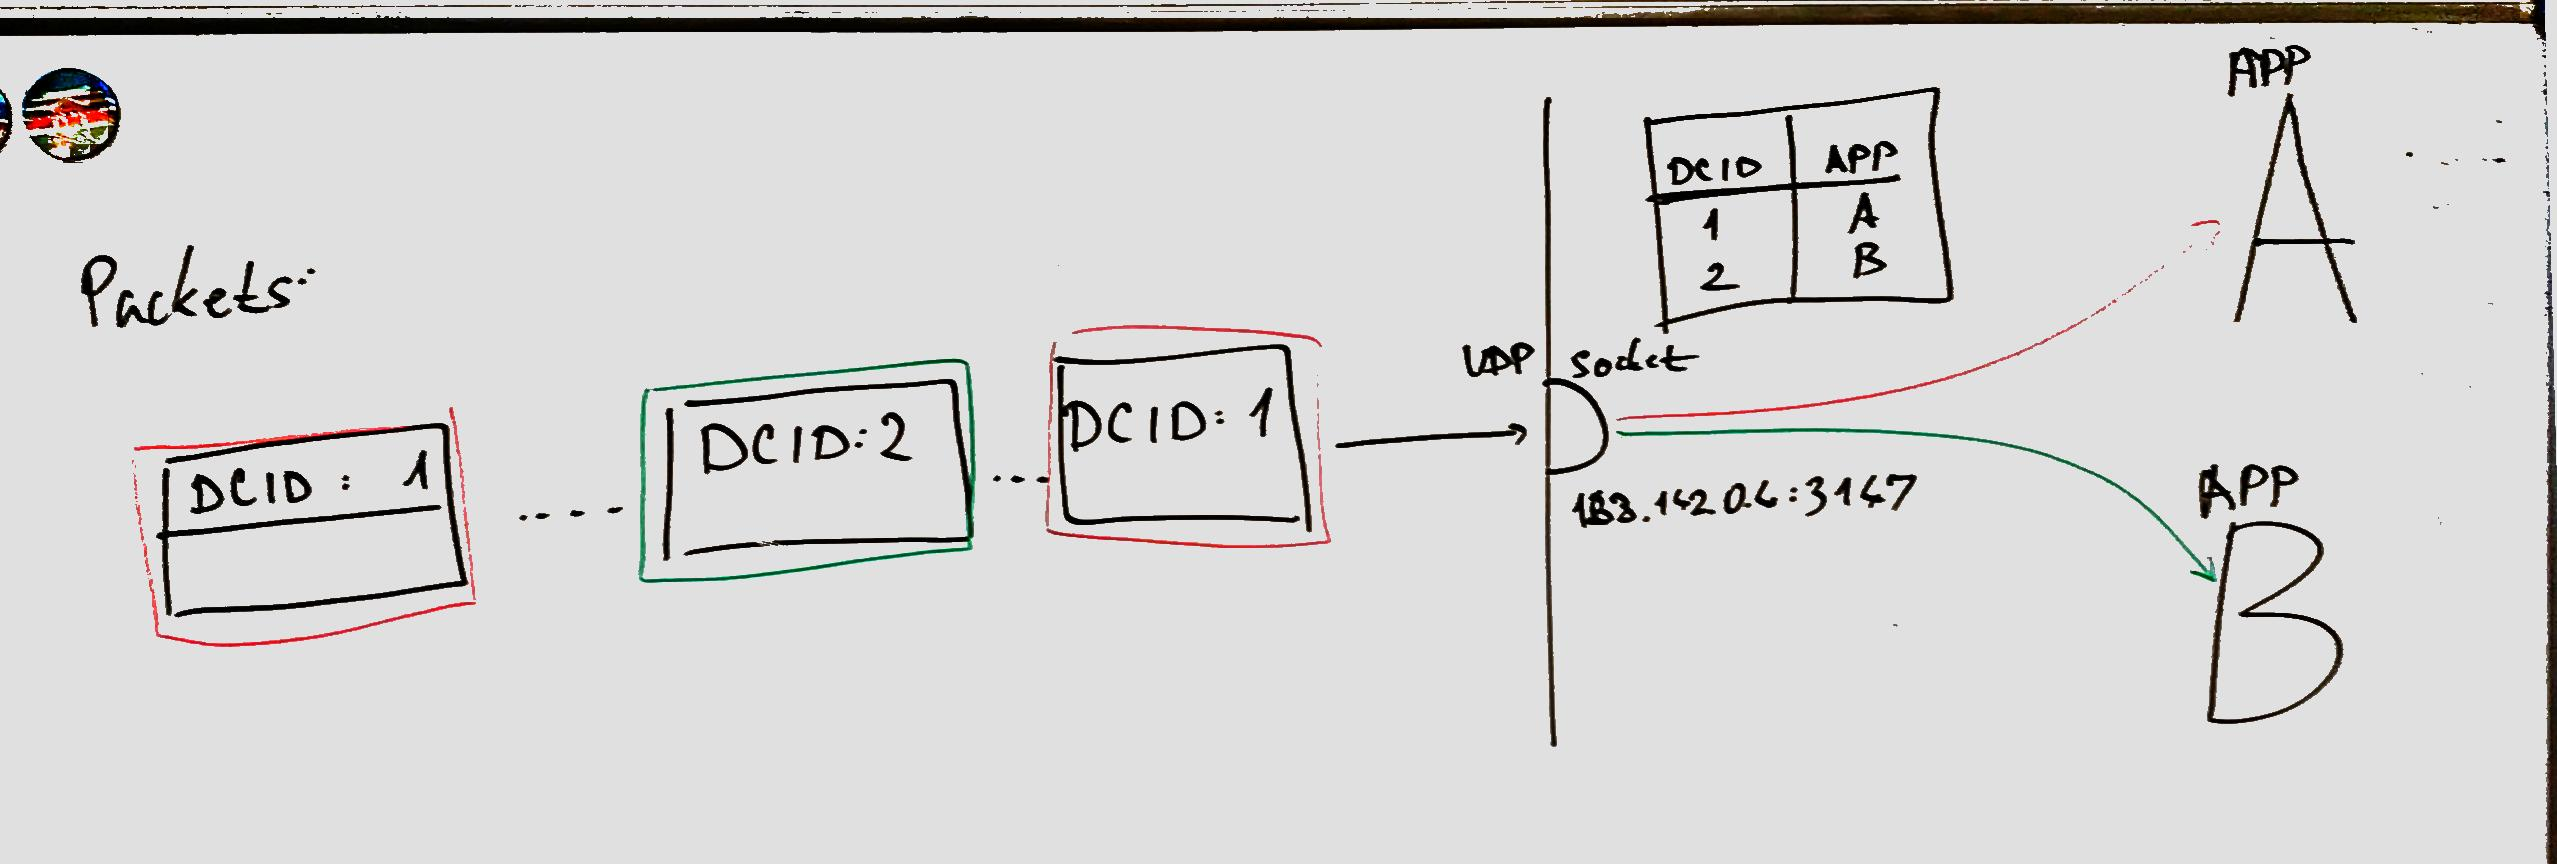
\includegraphics[width=0.9\textwidth]{img/02-socket-multiplexing}
\end{myFigure}

The payload of QUIC packets consists of one or more QUIC frames which carry individual pieces of
information such as acknowledgements or segments of the streams sent by the application.

QUIC can transport multiple streams in a single connection. These streams can be initiated by both
client and server, and can be either unidirectional, or bidirectional.
Figure~\ref{fig:02-stream-multiplexing} illustrates how QUIC may pack two streams into frames such
that those streams are transported in parallel.

\begin{myFigure}{fig:02-stream-multiplexing}{Stream multiplexing in QUIC}
  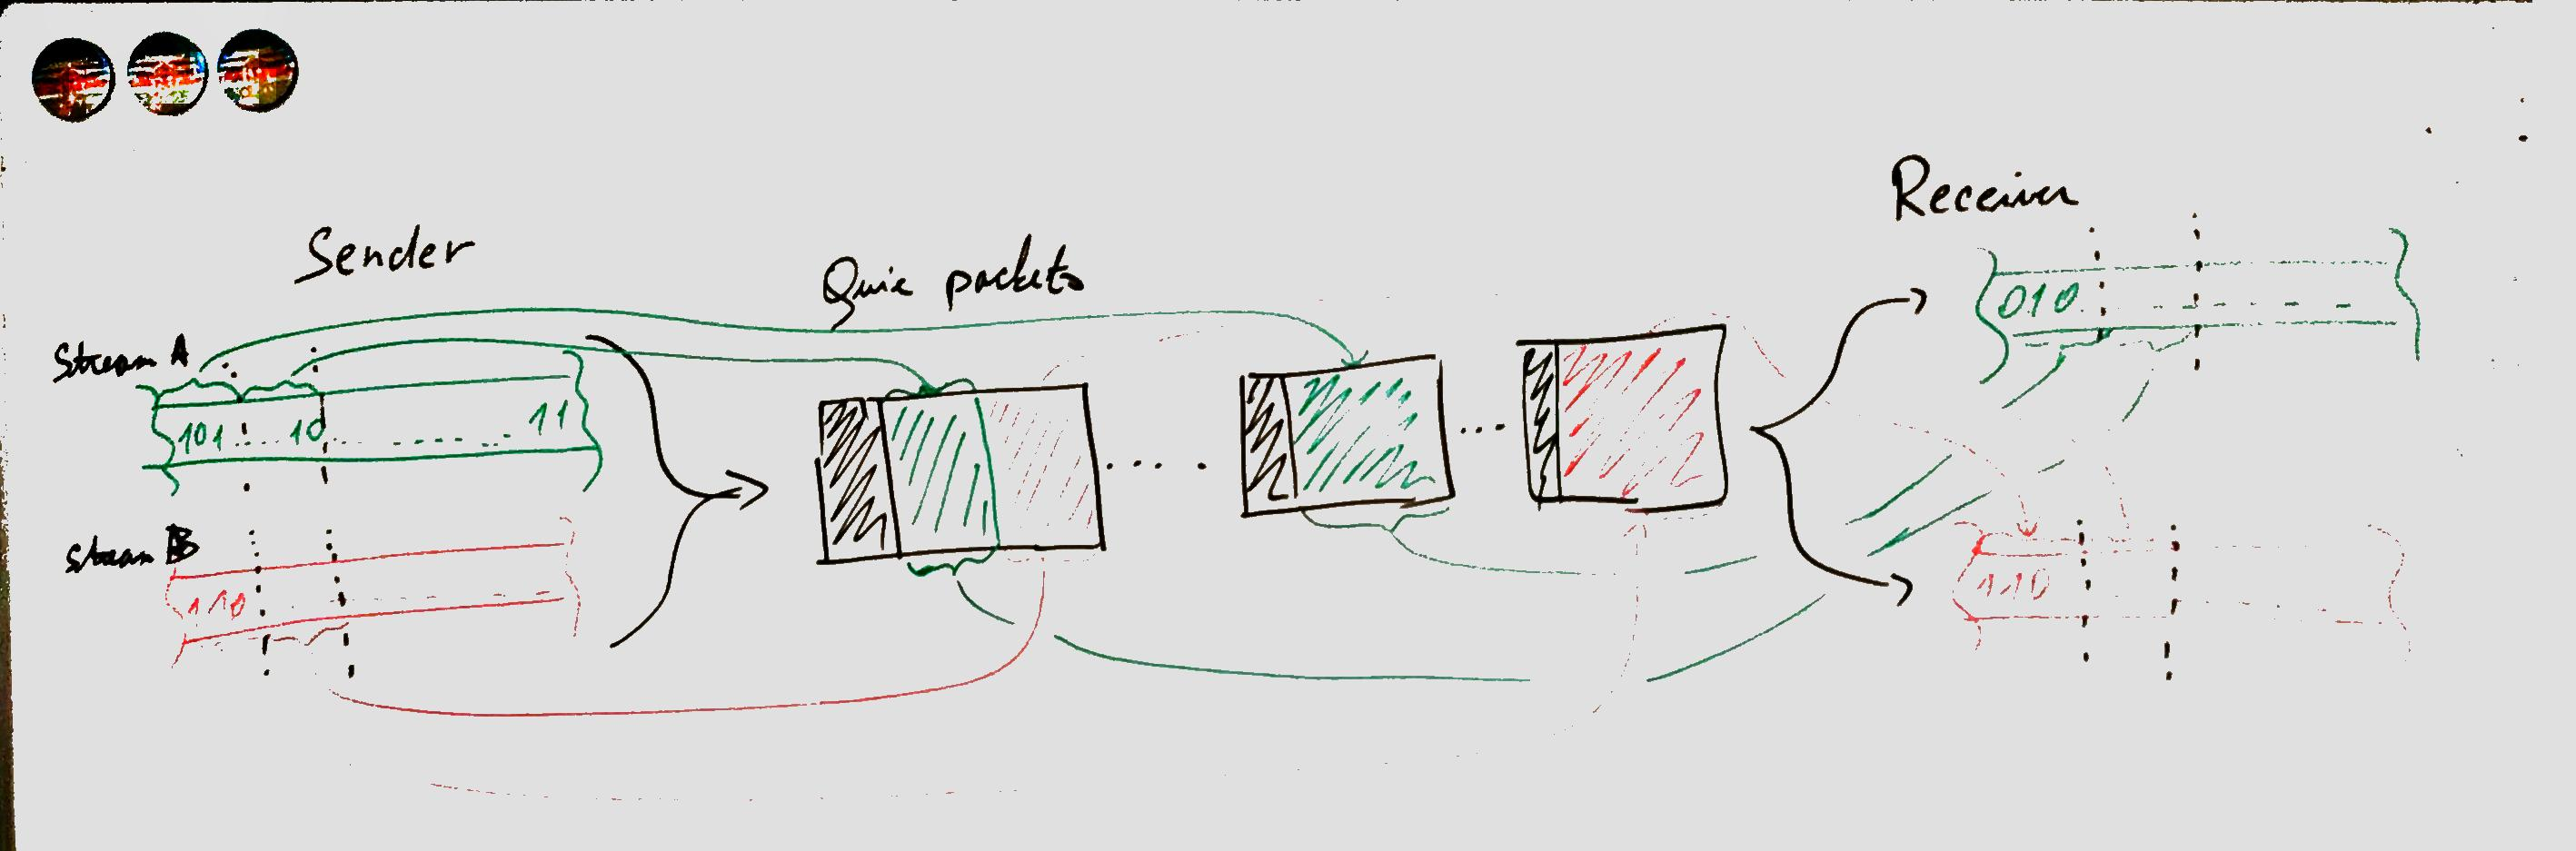
\includegraphics[width=0.9\textwidth]{img/02-stream-multiplexing}
\end{myFigure}

Similarly to TCP, packets in QUIC connections are numbered. However, QUIC uses three separate
\textit{Packet number spaces}:

\begin{enumerate}
  \litem{Initial} Used for exchanging initial information.
  \litem{Handshake} Used during the connection handshake process.
  \litem{1-RTT} Used throughout the lifetime of the connection to transfer application data.
\end{enumerate}

Packets from each packet number space are numbered and processed independently of the other packet
spaces. Each packet number space also uses different keys for encryption. Initial keys are derived
only from the Connection ID chosen by the client and therefore provide just an obfuscation. However,
the 1-RTT keys are negotiated by the TLS 1.3 protocol and offer high level of security. The packet
encryption is used for protection both against network traffic observers and against packet payload
corruption.

As a prevention against malicious too fast senders, QUIC implements a credit based flow-control
scheme. In this scheme, each peer advertises how much data it is willing to accept and how many
streams of each type can be opened by its peer. Violation of these limits leads to connection
termination.

Becuase UDP is an unreliable transport protocol, and QUIC must detect loss of the packets sent. The
loss detection is implemented similarly to TPC via acknowledgements of the received packets.
However, an important difference from TCP is that the lost packet is not retransmitted as-is.
Instead, the data carried by the lost packet are sent in different packets if necessary. This is
illustrated in figure~\ref{fig:02-packet-loss-example}

\begin{myFigure}{fig:02-packet-loss-example}{Retransmission of lost data in QUIC}
  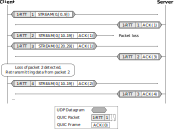
\includegraphics[width=0.6\textwidth]{img/02-retransmission-example}
\end{myFigure}

\section{Streams}

Streams transported by QUIC can be either unidirectional or bidirectional. Unidirectional streams
carry data from initiator to its peer, and bidirectional streams carry data in both directions.
Combined with distinguishing who initiated the stream, there are four types of streams:

\todo{explain the significance of lower 2 bits in the ID}

\begin{enumerate}

  \item \textit{Bidirectional client-initiated}
  \item \textit{Bidirectional server-initiated}
  \item \textit{Unidirectional client-initiated}
  \item \textit{Unidirectional server-initiated}.

\end{enumerate}

Each stream is identified by a unique \textit{Stream ID}, which is an integer between 0 and
$2^{62}-1$. \todo{maybe use ``62-bit unsigned integer'', remove the explanation why 62 bit, it is
  not necessary for this section} \todo{reader might wonder why such a big range, so maybe explain
  that the numbers are compressed and the number is just an upper limit} The maximum value of the stream ID is derived from the maximum value representable in
the particular binary encoding of integers on the wire, which will be described later in the
chapter. \todo{the example is not helpful, because the mapping to types is not evident} The 2 least significant bits of the Stream ID encode the type of the stream. For example,
client initiated unidirectional streams have Stream IDs 2, 6, 10 and so on.

Bidirectional streams can be viewed as two unidirectional streams combined together. After opening
the stream, each direction of the stream behaves as separate inbound and outbound unidirectional
streams, e.g.\@the reading and writing part of the stream can be closed independently of each other.

No special action needs to be taken by a peer who wishes to open a new stream. The peer can simply
start sending data. The stream can be then closed by writer either by specifying that all data has
been written to the stream, or by abruptly terminating the stream, also called \textit{resetting the
stream} in the specification. The reader of the stream can request stream reset in case it no longer
wishes to receive data on that stream. Abrupt termination of the stream requires specifying an
application-level error code that will be communicated to the peer.

QUIC specification specifies that the implementation should provide a way for application protocols
to specify relative priority of streams. \todo{This is impossible with current \dotnet{} API.}

The implementation should provide following operations on sending part of the stream:

\begin{itemize}

  \item write data;
  \item end the stream by specifying that all data has been written; and
  \item terminate the stream with an application-level error code.

\end{itemize}

On receiving part of the stream, application protocols need to be able to:

\begin{itemize}

  \item read data; and
  \item abort reading with an application-level error code.

\end{itemize}

\todo{mention or only link details of stream state machine?}

\section{Flow Control}

QUIC aims to be general-purpose transport protocol to be used over potentially untrusted network,
and as such it needs to protect endpoints from malicous peers. One of the mechanisms for achieving
this is limiting the amount of data sender can send and thus preventing overwhelming of slow
receivers by fast senders. Violations of the flow control limits result constitute a protocol
violation and result in an abrupt connection termination.

All QUIC streams are flow controlled individually, and also together as an aggregate. The receiver
controls the maximum amount of data sender can send by specifying

\begin{itemize}
  \item maximum offset of data sent for each individual streams and
  \item maximum sum of all offsets of data sent for individual streams.
\end{itemize}

Additionally, receiver also controls the maximum number of streams the sender can open at any given
moment in order to limit concurrency within a connection.

\section{Connection}

QUIC connections are made between two endpoints, with client endpoint initiating the connection to
the server endpoint. In a QUIC connection, endpoints exchange messages in the form of \textit{QUIC
packets}. QUIC packets are the smallest processable unit of the protocol, and are carried in UDP
datagrams. One UDP datagram can contain more than one QUIC packet, but QUIC packets cannot span
multiple UDP datagrams.

There are multiple QUIC packet types. These are following:

\begin{enumerate}
  \item \textit{Initial} and \textit{Handshake} --- used during connection establishment;
  \item \textit{1-RTT} --- main packets used during the lifetime of QUIC connection;
  \item \textit{Version Negotiation} --- sent by server when client tries to establish connection
    using unsupported version of QUIC\@;
  \item \textit{0-RTT} --- carries \textit{early data} similarly to TLS 1.3s \todo{feature name}
  \item \textit{Retry} --- used by servers during optional \todo{is it really optional?} client address validation.
\end{enumerate}

Payload of Initial, Handshake, and 1-RTT packets contains a sequence of \textit{frames} which are
the low-level messages of the QUIC protocol. Examples of frames include \texttt{STREAM} frames
carrying stream data, \texttt{ACK} frames carrying acknowledgements of received packets and
\texttt{CRYPTO} frames carrying cryptography negotiation messages.
Figure~\ref{fig:streams-frames-and-packets} illustrates how stream data are packaged in frames and
transmitted in packets.

\begin{figure}[h]\label{fig:streams-frames-and-packets}
  \centering
  \todo{sender, 2 colored streams, splitting to chunks to be carried in frames, STREAM and ACK
    frames in packets, unpacked at receiver}
\end{figure}

QUIC connections are identified by a connection ID, which is an opaque sequence of 8 to 20 bytes.
Each endpoint sets a value for its peer to include in packets sent towards the endpoint. The
separation of connection identification from endpoint's address eventually allows connection
migration.

\subsection{Handshake and Establishing a Connection}

As mentioned in the introduction, QUIC connection handshake combines TCP's three-way handshake with
TLS protocol handshake. This is achieved by carrying handshake messages of the TLS protocol in
\texttt{CRYPTO} frames. The content of the \texttt{CRYPTO} frames should not be interpreted by QUIC,
only passed to TLS implementation. TLS protocol is also used to negotiate QUIC protocol parameters
via TLS extension parameters and the application-level protocol is negotiated using ALPN
\todo{explain what ALPN is?} protocol.

Similarly to TLS, QUIC packets use increasingly more secure
protection keys for packet encryption.

\begin{itemize}
  \item \textit{Initial keys} are derived from protocol version and Destination Connection ID chosen
    by the client, and are more of an obfuscation rather than protection.
  \item \textit{Handshake keys} are derived during protection secrets exchange by the TLS layer and
    offer intermediate protection.
  \item \textit{1-RTT keys} are derived at the end of TLS handshake and offer strongest
    cryptographic protection.
\end{itemize}

The primary intent of Initial and Handshake packets is transport of \texttt{CRYPTO} frames


Clients initiate new connections by sending an \textit{Initial} QUIC packet. The packet contains a
header with version identifier and random \todo{at least outwardly} source\footnote{Even though
client here chooses both connection IDs, server is allowed choose new destination connection ID to
use and client must accept the change.} and destination connection ID\@. The client inititial packet
carry mainly \texttt{CRYPTO} frames containing TLS \textit{ClientHello} message.

Server replies to the clients initial by sending two packets: Initial packet with an \texttt{ACK}
frame acknowledging the receipt of the clients Initial; and Handshake packet with

\begin{enumerate}
  \item \textit{Version} --- identifier of the version of the protocol used;
  \item \textit{Source Connection ID} and \textit{Destination Connection ID} --- generated randomly
    in a way that can't be predicted by outside observer;
  \item \textit{}
\end{enumerate}

For performance reasons, implementations must the size of UDP datagrams sent in order to avoid
fragmentation at lower network layers. Loss or corruption of a single fragment would lead to entire
UDP datagram being discarded at receivers side. The maximum size, also called maximum transmission
unit (MTU) is dependent on the network and is generally around 1350 bytes.

\subsection{Connection Lifetime}

QUIC packets sent during the connection lifetime are strictly separated into three epochs, called
\textit{packet number spaces} in the specification. QUIC uses slightly different types of packets
for each packet number spaces, and we will refer to packet number spaces using the type of the
packet used in them: \textit{Initial}, \textit{Handshake} and \textit{1-RTT}. The packet number
spaces can be viewed as individual stages of connection establishment.

Packets sent in one packet number space are processed independently of the other packet number
spaces. For example, Acknowledgements for packets sent in \textit{Initial} epoch can only be only
sent in an \textit{Initial} packet. The three packet types also use different protection keys for
packet encryption:

\begin{itemize}

  \item \textit{Initial} --- Keys are derived solely from the protocol version used and the
    Connection ID chosen by the client. This protection is not considered secure, but merely an
    obfuscation.

  \item \textit{Handshake} --- Intermediate protection keys are derived by TLS implementation during
    encryption negotiation and provide partial protection.

  \item \textit{1-RTT} --- Fully secure protection keys are available after finishing connection.
    handshake.

\end{itemize}

Since only 1-RTT packet number space is considered secure, application data can only generally sent
only after connection handshake in 1-RTT packet number space. However, QUIC can optionally allow
sending application data in special \textit{0-RTT} packets. 0-RTT packets belong to 1-RTT packet
number space, but can be sent by client before receiving any packets from server. 0-RTT packet
support requires previous successful connection, and introduces a trade-off between reduced latency
and security.

\begin{itemize}

  \item Streams
  \item Flow control

  \item Connection
    \begin{itemize}
      \item Connection ID,
      \item Packets + Frames intro
      \item Connection establishment
        \begin{itemize}
          \item Encryption + TLS interleaving
          \item  handshake etc.
          \item Other security measures (peer validation)
        \end{itemize}
      \item transport parameters
      \item Connection Termination
    \end{itemize}
  \item Version negotiation
  \item Security
    \begin{itemize}
      \item Other security measures (peer validation)
    \end{itemize}
  \item Packets + Frames
  \item Generating acknowledgements + Recovery

  \item Connection migration?

  \item Detecting maximum packet size
  \item Encoding,
    \begin{itemize}
      \item Variable-length integer
      \item Packet headers, packets, frames, transport parameters
    \end{itemize}

\end{itemize}
